\documentclass[a4paper, 11pt]{article}
\usepackage[french]{babel}
\usepackage[utf8]{inputenc} 
\usepackage[T1]{fontenc}
\usepackage{multirow, multicol}
\usepackage{amsmath, amssymb, latexsym}
\usepackage{graphicx, epsfig,subfigure}
\usepackage[lined,boxed]{algorithm}
\usepackage{algorithmic}
\usepackage{rotate}
\usepackage{url}
\usepackage{setspace}
\usepackage{fancyhdr}

\newtheorem{definition}{Definition}
\newtheorem{example}{Example}
\newtheorem{proposition}{Proposition}
\newtheorem{proof}{Proof}
\pagestyle{fancy}
\fancyhf{}
\newcommand{\univ}{
\epsfig{file = logoUni.png, height = 1.05cm}}
\lhead{\univ}
\rhead{\date{\today}}
\rfoot{Page \thepage}

\title{}
\author{CHAMPENOIS Brandon \textsc{G5B} \\ BONVARLET Bastien \textsc{G5B} \\ MASSON Joris \textsc{G5B} }

\begin{document}
\maketitle
\centerline{
\includegraphics[width = 7cm]{ecos.png}}
\tableofcontents
\newpage

\section{rapide présentation / résumé du projet}


\newpage

\section{qui a fait quoi ?}

Bonvarlet bastien :\\
Masson Joris : \\
Champenois Brandon : Le menu du jeu, le rapport latex, les sprites de chaques entitées

\subsection{résumé de ce qui a était fait durant les semaines du projet}

Bonvarlet Bastien : \\
Masson Joris : \\
Champenois Brandon : Durant les 3 premières semaines j'ai fait tout les sprites de notre simulation d'écosystème, ensuite durant un peu plus d'un mois j'ai fait la fenetre de menu du jeu, et Enfin j'ai commencé le Latex le "28 mars 2022" et je l'ai fini le " ".
\newpage

\section{les difficultées rencontrées}

Nous avons eu quelques difficultées sur :

\newpage

\section{les eventuels ajout qu'on aurait voulu}

Si nous aurions eu plus de temps nous aurions voulu faire des fins alternatives et d'autres fenetres comme une fenetre de parametres.

\newpage

\section{les eventuels sources}

Pour les sprites : nous n'avons pas de sources puisqu'ils ont étaient fait par nos soins.
Pour la texture de la map :
Pour "l'algorithme" :
Pour le code :

\newpage

\section{conclusion}

Pour conclure nous aurions aimaient / voulu :

\newpage

\begin{figure*}[ht!]
 \centering
 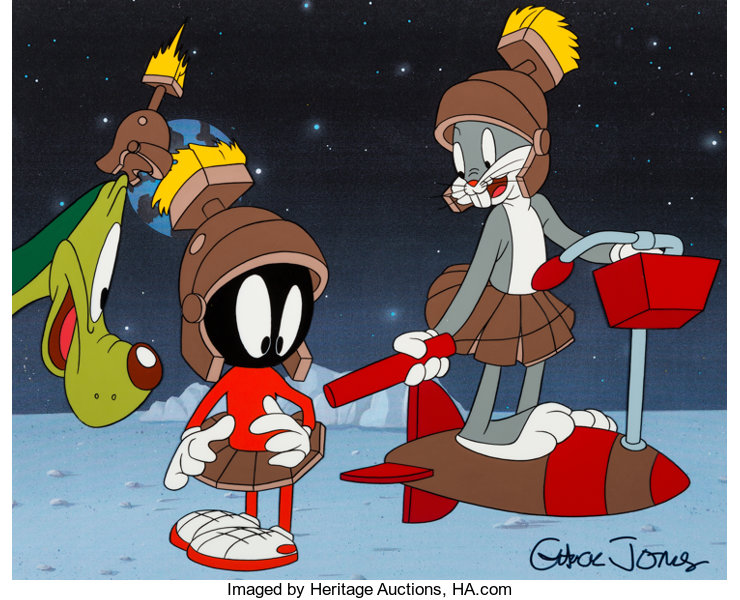
\includegraphics[width=0.7\linewidth]{picture.jpg}
 \caption{Go head punk, make my day}
 \label{fig::example::one}
\end{figure*}

\begin{multicols}{2}
Now that we know who you are, I know who I am. I'm not a mistake! It all makes sense! In a comic, you know how you can tell who the arch-villain's going to be? He's the exact opposite of the hero.
\begin{example}
It actually says that in the little book that comes with it: the most popular gun in American crime. Like they're actually proud of that shit. 
\end{example}
\end{multicols}

That's clear.

\begin{itemize}
 \item Your cells 
 \item react to bacteria and viruses 
 \item differently than mine.
\end{itemize}

\begin{table}
 \centering
 \begin{tabular}{|c|c|c|}
  \hline
  & \textbf{Shot} & \textbf{Hide}\\\hline
  \textbf{Marcellus} & $m(1 - m)$ & $m^2$\\
  \textbf{Winston} & $(1 - m)^2$ & $m(1 - m)$\\\hline
 \end{tabular}
 \caption{Do you see any Teletubbies in here?}
 \label{tab::tubbies}
\end{table}

\begin{figure*}[ht!]
  \begin{minipage}[c]{.49\linewidth}
   \centering
   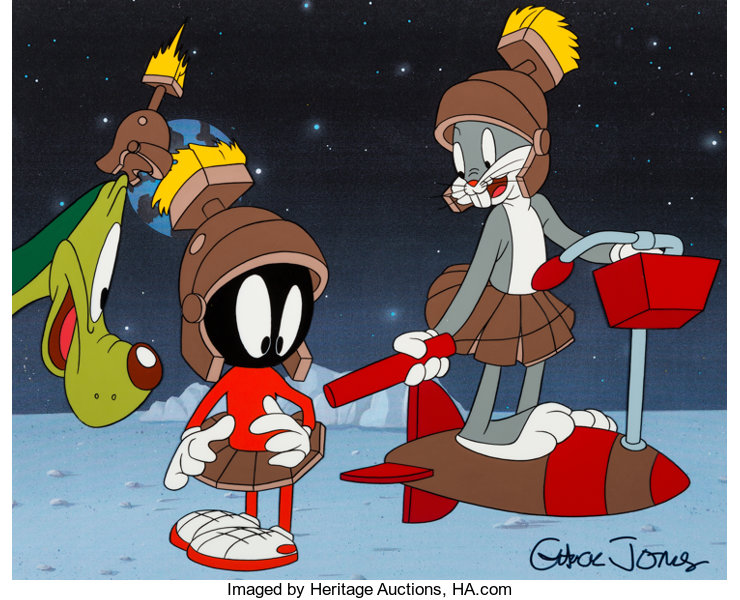
\includegraphics[width=\linewidth]{picture.jpg}
  \end{minipage} \hfill
  \begin{minipage}[c]{.49\linewidth}
   \centering
   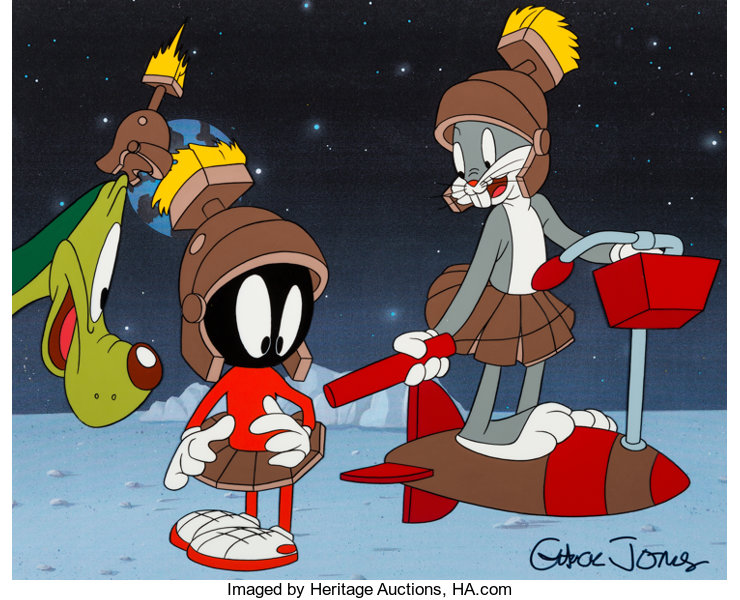
\includegraphics[width=\linewidth]{picture.jpg}
  \end{minipage}
  \caption{(a) Hey!; (b) Go head punk}
  \label{fig::example::two}
\end{figure*}

\begin{enumerate}
 \item The path of the righteous man is beset on all sides by the iniquities of the selfish and the tyranny of evil men. 
 \item Blessed is he who, in the name of charity and good will, shepherds the weak through the valley of darkness, for he is truly his brother's keeper and the finder of lost children. 
 \item And I will strike down upon thee with great vengeance and furious anger those who would attempt to poison and destroy My brothers. 
 \item And you will know My name is the Lord when I lay My vengeance upon thee.
\end{enumerate}
\end{document}
